\documentclass[
	a4paper,
	oneside,
	DIV = 12,
	12pt,
	headings = normal,
]{scrartcl}

%%% Support for color
\usepackage{xcolor}
\definecolor{lightblue}{HTML}{03A9F4}
\definecolor{red}{HTML}{F44336}
%%%

%%% Including graphics
\usepackage{graphicx}
%%%

%%% Font selection
\usepackage{fontspec}

\setromanfont{STIX Two Text}[
	SmallCapsFeatures = {LetterSpace = 5},
]

\setsansfont{Source Sans Pro}[
]

\setmonofont{Source Code Pro}[
]
%%%

%%% Math typesetting
\usepackage{amsmath}
\usepackage{mathtools}
\usepackage{unicode-math}
\setmathfont{STIX Two Math}

\usepackage[retainorgcmds]{IEEEtrantools}

\DeclarePairedDelimiter{\ceil}{\lceil}{\rceil}

\newcommand*\lnand{\mathbin{\barwedge}}
%%%

%%% Font settings for different KOMAScript elements
\setkomafont{pagenumber}{\rmfamily}
\setkomafont{disposition}{\rmfamily\bfseries}
%%%

%%% Typographic enhancements
\usepackage{microtype}
%%%

%%% Language-specific settings
\usepackage{polyglossia}
\setmainlanguage{ukrainian}
%%%

%%% Captions
\usepackage{caption}
\usepackage{subcaption}

\DeclareCaptionLabelFormat{closing}{#2)}
\captionsetup[subtable]{labelformat = closing}
\captionsetup[subfigure]{labelformat = closing}
%%%

%%% Table typesetting
\usepackage{booktabs}
\usepackage{longtable}

\usepackage{multirow}

\usepackage{array}
\newcolumntype{v}[1]{>{\raggedright\arraybackslash\hspace{0pt}}p{#1}}
\newcolumntype{b}[1]{>{\centering\arraybackslash\hspace{0pt}}p{#1}}
\newcolumntype{n}[1]{>{\raggedleft\arraybackslash\hspace{0pt}}p{#1}}
%%%

%%% SI units typesetting
\usepackage{siunitx}
\sisetup{output-decimal-marker = {,},
exponent-product = {\cdot}}
%%%

%%% TIKZ
\usepackage{tikz}
\usetikzlibrary{arrows.meta, automata, calc, positioning, shapes}
\usetikzlibrary{paths.ortho}

\usepackage{tikzscale}
%%%

%%% Links and hyperreferences
\usepackage{hyperref}
\hypersetup{
	colorlinks      = false,
	linkbordercolor = red,
	urlbordercolor  = lightblue,
	pdfborderstyle  = {/S/U/W 1.5},
}
%%%

%%% Custom commands
\newcommand\schel[1]{\textit{#1}}

\newcommand{\barneg}[1]{\overline{#1}}
%%%

\begin{document}
	\begin{titlepage}
		\begin{center}
			Міністерство освіти і науки України\\
			Національний авіаційний університет\\
			Навчально-науковий інститут комп'ютерних інформаційних технологій\\
			Кафедра комп'ютеризованих систем управління

			\vspace{\fill}
				Розрахунково-графічна робота\\
				з дисципліни «Комп'ютерна схемотехніка»\\

			\vspace{\fill}

			\begin{flushright}
				Виконав:\\
				студент ННІКІТ\\
				групи СП-225\\
				Клокун Владислав\\
				Перевірив:\\
				Іскренко Ю. Ю.
			\end{flushright}

			Київ 2017
		\end{center}
	\end{titlepage}

	\section{Завдання}
		Завданням розрахунково-графічної роботи є розробка алгоритму виконання вказаної в завданні операції та синтезу функціональної схеми керуючого автомата.

		\begin{longtable}[c]{lr}
			\toprule
				Параметр & Значення\\
			\midrule
			\endhead
			\bottomrule
			\caption{Завдання на розрахунково-графічну роботу}
			\endfoot
			\label{tab:rgr-task}

			№                        & 16\\
			Тип операції             & Додавання\\
			Початковий код операндів & ДК\\
			Розрядність операндів    & 16\\
			КВМСМ                    & МДК\\
			Структура ОБ             & ЗМО\\
			Тип автомата             & Мілі\\
			Пам'ять автомата         & $D$\\
			ОР                       & $P$\\
			ЛО                       & \textit{NAND}\\
		\end{longtable}

		З завдання на розрахунково-графічну роботу (табл.~\ref{tab:rgr-task}) видні такі характеристики цільового арифметико-логічного пристрою:
		\begin{enumerate}
			\item Тип арифметичної операції — додавання двійкових чисел.
			\item Початковий код подання операндів~— доповняльний.
			\item Розрядність операндів — 16~біт.
			\item Код виконання операції у суматорі~— доповняльний модифікований.
			\item Структура операційного блока~— із закріпленими мікроопераціями.
			\item Тип керуючого блока~— автомат Мілі з пам'яттю на $D$-тригерах.
			\item Схема логічної ознаки парності молодшого байту.
		\end{enumerate}

	\section{Хід роботи}
		\subsection{Розробка алгоритму}
			Алгоритм додавання двійкових чисел можна словесно описати так:
			\begin{enumerate}
				\item У першому і другому машинних тактах із вхідної шини паралельним кодом записуються операнди~$A$ і~$B$ у відповідні регістри \schel{RGA} і \schel{RGB}. Зчитування операндів здійснюється ЦПК.
				\item Протягом одного машинного такту виконується мікрооперація додавання.
				\item Якщо розрядна сітка не переповнилась, результат записується у регістр~\schel{RGC}.
				\item Якщо розрядна сітка переповнилась, результат не фіксується, і в ЦПК подається сигнал переповнення «ПП».
			\end{enumerate}

		\subsection{Побудова граф-схем}
			У процесі виконання розрахунково-графічної роботи за алгоритмом була розроблена мікропрограма додавання~(її змістовний граф на рис.~\ref{fig:summation-algorithm-meaningful-graph}).
			\begin{figure}[!htbp]
			\centering
				\includegraphics{assets/01-summation-algorithm-meaningful-graph.tikz}
			\caption{Змістовний граф мікропрограми додавання}
			\label{fig:summation-algorithm-meaningful-graph}
			\end{figure}

			Далі отриманий на попередньому етапі змістовний граф мікропрограми був закодований і розмічений~(рис.~\ref{fig:summation-algorithm-encoded-graph}).

			\begin{figure}[!htbp]
			\centering
				\includegraphics{assets/02-summation-algorithm-encoded-graph.tikz}
			\caption{Закодований граф мікропрограми додавання}
			\label{fig:summation-algorithm-encoded-graph}
			\end{figure}

		\subsection{Синтез}
			За результатом кодування графа згідно відповідно до завдання був синтезований автомат Мілі~(рис.~\ref{fig:mealy-machine}).

			\begin{figure}[!htbp]
			\centering
				\includegraphics{assets/03-sum-mealy-machine.tikz}
			\caption{Граф автомата Мілі для мікропрограми додавання}
			\label{fig:mealy-machine}
			\end{figure}

			З синтезованого автомата Мілі видно, що максимальна кількість станів автомата~$L = 8$. Для реалізації такої кількості станів необхідно використати $n = \ceil*{\log_2{8}} = 3$~$D$-тригери.

			Закодуємо стани автомата Мілі значеннями виходів $D$-тригерів за принципом кодування Грея та зобразимо це відповідним чином на рисунку.
			\begin{IEEEeqnarray*}{rClrClrCl}
				z_1 &=& \barneg{Q_1} \barneg{Q_2} \barneg{Q_3}, \quad &
				z_2 &=& \barneg{Q_1} \barneg{Q_2}         Q_3, \quad &
				z_3 &=& \barneg{Q_1}         Q_2          Q_3,\\
				z_4 &=& \barneg{Q_1}         Q_2  \barneg{Q_1}, \quad &
				z_5 &=&         Q_3          Q_2  \barneg{Q_1}, \quad &
				z_6 &=&         Q_3          Q_2          Q_1,\\
				z_7 &=&         Q_3  \barneg{Q_2}         Q_1, \quad &
				z_8 &=&         Q_3  \barneg{Q_2} \barneg{Q_1}.
			\end{IEEEeqnarray*}

			% Будуємо таблицю переходів автомату Мілі~(табл.~\ref{tab:transfer-table}).

			% \begin{longtable}[c]{cccccccccccccccccccc}
				% \toprule
					% \multicolumn{4}{c}{$t$} & \multicolumn{15}{c}{$t+1$}\\
					% \cmidrule(lr){1-3} \cmidrule(lr){4-20}
					% $Q_1Q_2Q_3$ & $\beta_1$ & $x_1$ & $Q_1Q_2Q_3$ & $y_1$ & $y_2$ & $y_3$ & $y_4$ & $y_5$ & $y_6$ & $y_7$ & $y_8$ & $y_9$ & $D_1D_2D_3$\\
				% \midrule
				% \endhead
				% \bottomrule
				% \caption{Таблиця переходів автомата}
				% \endfoot
				% \label{tab:transfer-table}

					% $000$ & $1$ & $—$ & $000$ & $0$ & $0$ & $0$ & $0$ & $0$ & $0$ & $0$ & $0$ & $0$ & $000$\\
					% $000$ & $—$ & $—$ & $001$ & $1$ & $0$ & $0$ & $0$ & $0$ & $0$ & $0$ & $0$ & $0$ & $001$\\
					% $001$ & $—$ & $—$ & $011$ & $0$ & $1$ & $0$ & $0$ & $0$ & $0$ & $0$ & $0$ & $0$ & $011$\\
					% $011$ & $—$ & $—$ & $010$ & $0$ & $0$ & $1$ & $0$ & $0$ & $0$ & $0$ & $0$ & $0$ & $010$\\
					% $010$ & $—$ & $—$ & $110$ & $0$ & $0$ & $0$ & $1$ & $0$ & $0$ & $0$ & $0$ & $0$ & $110$\\
					% $110$ & $—$ & $—$ & $111$ & $0$ & $0$ & $0$ & $0$ & $1$ & $0$ & $0$ & $0$ & $0$ & $111$\\
					% $111$ & $—$ & $—$ & $101$ & $0$ & $0$ & $0$ & $0$ & $0$ & $1$ & $0$ & $0$ & $0$ & $101$\\
					% $101$ & $—$ & $1$ & $000$ & $0$ & $0$ & $0$ & $0$ & $0$ & $0$ & $0$ & $0$ & $1$ & $000$\\
					% $101$ & $—$ & $0$ & $100$ & $0$ & $0$ & $0$ & $0$ & $0$ & $0$ & $1$ & $0$ & $0$ & $100$\\
					% $100$ & $—$ & $—$ & $000$ & $0$ & $0$ & $0$ & $0$ & $0$ & $0$ & $0$ & $1$ & $0$ & $000$\\
			% \end{longtable}

			Для наочності складемо структурну таблицю переходів автомату Мілі~(табл.~\ref{tab:structured-transfer-table}).
			\begin{longtable}[c]{ccccccccc}
				\toprule
					$z_i$ & $k(z_i)$ & $z_j$ & $k(z_j)$ & $\left\{ x_i \right\}$ & $\left\{ y_i \right\}$ & $D_1$ & $D_2$ & $D_3$\\
				\midrule
				\endhead
				\bottomrule
				\caption{Структурна таблиця переходів автомата Мілі}
				\endfoot
				\label{tab:structured-transfer-table}

					$z_1$ & $000$ & $z_1$ & $000$ & $\barneg{\beta_1}$ & $—$   & $0$ & $0$ & $0$\\
					$z_1$ & $000$ & $z_2$ & $001$ & $1$                & $y_1$ & $0$ & $0$ & $1$\\
					$z_2$ & $001$ & $z_3$ & $011$ & $1$                & $y_2$ & $0$ & $1$ & $1$\\
					$z_3$ & $011$ & $z_4$ & $010$ & $1$                & $y_3$ & $0$ & $1$ & $0$\\
					$z_4$ & $010$ & $z_5$ & $110$ & $1$                & $y_4$ & $1$ & $1$ & $0$\\
					$z_5$ & $110$ & $z_6$ & $111$ & $1$                & $y_5$ & $1$ & $1$ & $1$\\
					$z_6$ & $111$ & $z_7$ & $101$ & $1$                & $y_6$ & $1$ & $0$ & $1$\\
					$z_7$ & $101$ & $z_1$ & $000$ & $x_1$              & $y_9$ & $0$ & $0$ & $0$\\
					$z_7$ & $101$ & $z_8$ & $100$ & $\barneg{x_1}$     & $y_7$ & $1$ & $0$ & $0$\\
					$z_8$ & $100$ & $z_1$ & $000$ & $1$                & $y_8$ & $0$ & $0$ & $0$\\
			\end{longtable}

			На підставі даних структурної таблиці переходів автомату Мілі записуємо системи логічних рівнянь. Для функцій збудження входів:
			\begin{IEEEeqnarray*}{rCl}
				D_1 &=& z_4 \lor z_5 \lor z_6 \lor z_7 \barneg{x_2},\\
				D_2 &=& z_2 \lor z_3 \lor z_4 \lor z_5,\\
				D_3 &=& z_1 \lor z_2 \lor z_5 \lor z_6.
			\end{IEEEeqnarray*}

			Перетворимо отримані функції до заданого у завданні елементного базису NAND («І—НЕ», тут і далі позначається символом~$\lnand$):
			\begin{IEEEeqnarray*}{rCl}
				D_1 &=& z_4 \lor z_5 \lor z_6 \lor z_7 \barneg{x_2}
				    = \barneg{z_4} \lnand \barneg{z_5} \lnand \barneg{z_6} \lnand \left( z_7 \lnand x_2 \right),\\
				D_2 &=& z_2 \lor z_3 \lor z_4 \lor z_5
				    = \barneg{z_2} \lnand \barneg{z_3} \lnand \barneg{z_4} \lnand \barneg{z_5},\\
				D_3 &=& z_1 \lor z_2 \lor z_5 \lor z_6
				    = \barneg{z_1} \lnand \barneg{z_2} \lnand \barneg{z_5} \lnand \barneg{z_6}.
			\end{IEEEeqnarray*}

			Для вихідних сигналів:
			\begin{IEEEeqnarray*}{rClrClrCl}
				y_1 &=& z_1, \quad &
				y_2 &=& z_2, \quad &
				y_3 &=& z_3, \\
				y_4 &=& z_4, \quad &
				y_5 &=& z_5, \quad &
				y_6 &=& z_6, \\
				y_7 &=& z_7 \barneg{x_1}, \quad &
				y_8 &=& z_8, \quad &
				y_9 &=& z_7 x_1.
			\end{IEEEeqnarray*}

			В результаті розробили функціональну схему керуючого автомату~(рис.~\ref{fig:control-automata-schematic}).

			\begin{figure}[!htbp]
			\centering
				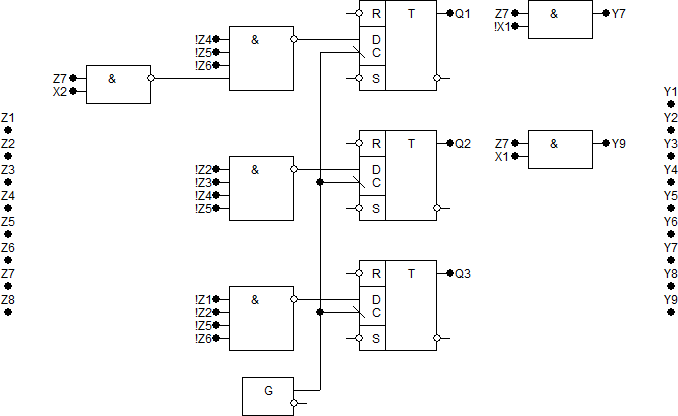
\includegraphics[height = 16\baselineskip]{assets/control-schematic.png}
			\caption{Функціональна схема керуючого автомата}
			\label{fig:control-automata-schematic}
			\end{figure}

	\section{Висновок}
		Під час виконання даної розрахунково-графічної роботи ми навчились розробляти мікропрограми для виконання арифметично-логічних операцій, синтезувати за розробленим алгоритмом відповідні керуючі автомати та реалізовувати синтезовані автомати у вигляді функціональних схем.

\end{document}
